\documentclass[pra,12pt]{revtex4}
\usepackage{amsmath}
\usepackage{amssymb}
\usepackage{graphicx}
\usepackage{color}
\usepackage{enumerate}
\usepackage{framed}
\usepackage[pdfborder={0 0 0},colorlinks=true,linkcolor=blue,urlcolor=blue]{hyperref}

\def\ket#1{\left|#1\right\rangle}
\def\bra#1{\left\langle#1\right|}
\def\braket#1{\left\langle#1\right\rangle}

\usepackage{fancyhdr}
\fancyhf{}
\lhead{\tiny Y.~D.~Chong}
\rhead{\scriptsize PH4401: Quantum Mechanics III}
\lfoot{}
\rfoot{\thepage}
\pagestyle{fancy}

\renewcommand{\theequation}{1.\arabic{equation}}

\setlength{\parindent}{14pt}

\renewcommand{\baselinestretch}{1.0}
\setlength{\parskip}{0.07in}

\def\thesection{1.\arabic{section}}
\def\thesubsection{1.\arabic{section}.\arabic{subsection}}

\begin{document}

\begin{center}
{\Large \textbf{Chapter 1: Scattering Theory}}
\end{center}

%% \section{Scattering Processes in Quantum Mechanics}

\section{Scattering experiments on quantum particles}

Quantum particles exhibit a feature known as \textbf{wave-particle
  duality}, which can be summarized in the \textbf{quantum double-slit
  thought experiment}.  As illustrated below, a source emits electrons
of energy $E$ toward a screen with a pair of slits.  A movable
detector is placed on the far side, to measure the arrival rates at
different positions.

\begin{figure}[h]
  \centering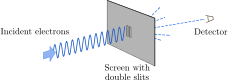
\includegraphics[width=0.6\textwidth]{doubleslit}
\end{figure}

The experiment reveals the following: (i) the electrons arrive in
discrete units, like classical particles; (ii) the
\textit{statistical} distribution of electron arrivals forms an
interference pattern, like a diffracted wave.  In the non-relativistic
limit, the inferred wavelength $\lambda$ is related to the electron
energy $E$ by
\begin{equation}
  \lambda = \frac{2\pi}{k}, \;\;\; E = \frac{\hbar^2k^2}{2m},
\end{equation}
where $\hbar = h/2\pi$ is Dirac's constant, and $m$ is the electron
mass.  (This means that if $E$ is known, we can deduce the spacing of
the slits by studying the diffraction pattern.)

Wave-particle duality arises from quantum theory's distinction between
a particle's state and the outcomes of measurements performed on it.
The state is described by a wavefunction $\psi(\mathbf{r})$, which can
undergo diffraction like a classical wave.  On the other hand, the
probability of measuring a particle in a volume $dV$ around position
$\mathbf{r}$ is given by $|\psi(\mathbf{r})|^2 \,dV$.

In this chapter, we will study a generalization of the double-slit
experiment called a \textbf{scattering experiment}.  The idea is to
shoot quantum particles at a target, called a \textbf{scatterer}, and
measure the distribution of scattered particles.  Just as the
double-slit interference pattern can be used to deduce the slit
spacing, a scattering experiment can be used to deduce various facts
about the scatterer.  Scattering experiments constitute a large
proportion of the methods used to probe the quantum world, from
electron- and photon-based microscopy to accelerator experiments in
high-energy physics.

We will focus on the non-relativistic scattering experiment depicted
in the figure below.  An unbounded $d$-dimensional space is described
by coordinates $\mathbf{r}$, with a scatterer near $\mathbf{r} = 0$.
An incoming quantum particle, with energy $E$, is governed by the
Hamiltonian
\begin{equation}
  \hat{H} = \hat{H}_0 + V(\hat{\mathbf{r}}), \;\;\;
  \hat{H}_0 = \frac{\hat{\mathbf{p}}^2}{2m},
\end{equation}
where $\hat{H}_0$ describes the particle's kinetic energy, $m$ is the
particle's mass, $\hat{\mathbf{r}}$ and $\hat{\mathbf{p}}$ are
position and momentum operators, and $V$ is a \textbf{scattering
  potential} describing how the scatterer affects the quantum
particle.  We assume that $V(\mathbf{r}) \rightarrow 0$ as
$|\mathbf{r}| \rightarrow \infty$.

\begin{figure}[h]
  \centering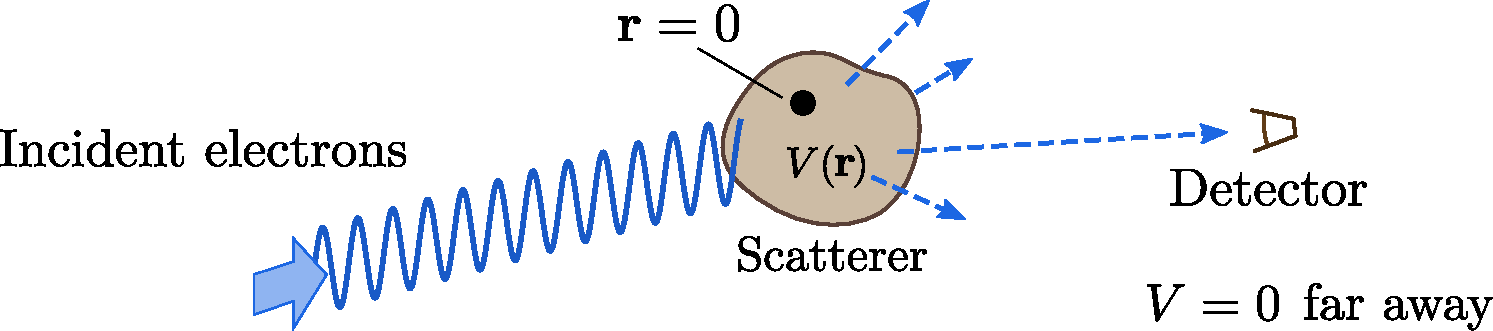
\includegraphics[width=0.68\textwidth]{scattering}
\end{figure}

We want to see how this particle is scattered by the potential.  But
how can the above description be formulated as a well-posed problem?
Let us give the formulation first, before discussing its meaning:
\begin{enumerate}
\item 
The particle state $|\psi\rangle$ obeys the time-independent
Schr\"odinger equation
\begin{equation}
  \hat{H} |\psi\rangle = E |\psi\rangle,
\end{equation}
where $E$ is the incoming particle energy.

\item
This state can be decomposed into two terms,
\begin{equation}
  |\psi\rangle \,=\, |\psi_i\rangle \,+\, |\psi_s\rangle,
\end{equation}
where $|\psi_i\rangle$ is called the \textbf{incident state} and
$|\psi_s\rangle$ is called the \textbf{scattered state}.

\item
The incident state is described by a plane wave---a simultaneous
eigenstate of $\hat{H}_0$ (with energy $E$) and $\hat{\mathbf{p}}$
(with momentum $\mathbf{p}_i$):
\begin{equation}
  \hat{H}_0 |\psi_i\rangle = E |\psi_i\rangle \;\; \mathrm{and}\;\;
  \hat{\mathbf{p}} |\psi_i\rangle = \mathbf{p}_i |\psi_i\rangle,
  \;\; \mathrm{where}\;\; E = \frac{|\mathbf{p}_i|^2}{2m}.
\end{equation}

\item
The scattered state is an ``outgoing'' state.  What this means will be
explained later.
\end{enumerate}
We can interpet the above conditions as follows.  Condition 1 says
that the scattering process is elastic: since the scatterer is
described by a potential $V(\mathbf{r})$, its interaction with the
particle is conservative, so $E$ is fixed.  Condition 2 says that the
particle's wavefunction $\psi(\mathbf{r}) = \langle \mathbf{r}
|\psi\rangle$ is a superposition of an incoming wave and a scattered
wave.  Condition 3 defines the incoming wave as a plane wave with
wavelength determined by $E$.  Finally, condition 4 says that the wave
moves outward to infinity after being scattered.

Note that \textit{this is not an eigenproblem}!  Usually, the
time-independent Schr\"odinger equation is treated as an eigenproblem
(i.e., we solve for eigenvalues and eigenstates).  Here, we are given
$|\psi_i\rangle$, $E$, and $V(\mathbf{r})$, and we want
$|\psi_s\rangle$.  In particular, $E$ is an input, not an output.

\section{Recap: position and momentum states}
\label{sec:waves}

Before proceeding, let us review the properties of quantum particles
in free space.  In a $d$-dimensional space, a coordinate vector
$\mathbf{r}$ is a real vector of $d$ components.  A quantum particle
can be described by the position basis---a set of quantum states
$\{|\mathbf{r}\rangle\}$, one for each possible $\mathbf{r}$.  If we
are studying a particle trapped in a finite region (e.g., a particle
in a box), $\mathbf{r}$ is restricted to that region; otherwise,
$\mathbf{r}$ is any real $d$-dimensional vector.  In either case, the
position labels are continuous so $\{|\mathbf{r}\rangle\}$ is an
uncountably infinite set.

The position eigenstates span the state space, so the identity
operator can be resolved as
\begin{equation}
  \hat{I} = \int d^dr \, |\mathbf{r}\rangle \,\langle\mathbf{r}|,
\end{equation}
where the integral is taken over all allowed $\mathbf{r}$.  It
follows that
\begin{equation}
  \langle \mathbf{r} | \mathbf{r}' \rangle = \delta^d(\mathbf{r}-\mathbf{r}').
\end{equation}
The position eigenstates are thus said to be ``delta normalized'',
rather than being normalized to unity.  Here, $\delta^d(\cdots)$
denotes the $d$-dimensional delta function; e.g., in 2D,
\begin{equation*}
  \langle x,y \,|\, x',y' \rangle = \delta(x-x') \, \delta(y-y').
\end{equation*}
The position operator $\hat{\mathbf{r}}$ is defined such that
$|\mathbf{r}\rangle$ and $\mathbf{r}$ are its eigenstates and
eigenvalues:
\begin{equation}
  \hat{\mathbf{r}} |\mathbf{r}\rangle \,=\, \mathbf{r}\, |\mathbf{r}\rangle.
\end{equation}

Momentum eigenstates are constructed from position eigenstates via
Fourier transforms.  First, suppose the allowed region of space is a
box of length $L$ on each side, with periodic boundary conditions.
Define the set of wave-vectors
\begin{equation*}
  \Big\{\mathbf{k}  \; \Big| \;\; k_j = 2\pi m/L\;\;\mathrm{for}
  \;m\in\mathbb{Z}, \; j = 1, \dots,d\, \Big\},
\end{equation*}
corresponding to plane waves satisfying the periodic boundary
conditions.  Now define
\begin{equation}
  |\mathbf{k}\rangle = \frac{1}{L^{d/2}} \, \int d^dr \; e^{i\mathbf{k}\cdot\mathbf{r}} |\mathbf{r}\rangle,
\end{equation}
where the integral is taken over the box.  These can be shown to
satisfy
\begin{equation}
  \langle\mathbf{k}|\mathbf{k}'\rangle = \delta_{\mathbf{k},\mathbf{k}'}, \quad \langle\mathbf{r}|\mathbf{k}\rangle = \frac{1}{L^{d/2}} e^{i\mathbf{k}\cdot\mathbf{r}}, \quad I = \sum_{\mathbf{k}} |\mathbf{k}\rangle\,\langle\mathbf{k}|.
\end{equation}
The momentum operator is defined to have each $|\mathbf{k}\rangle$ is
an eigenstate, with eigenvalue $\hbar\mathbf{k}$:
\begin{equation}
  \hat{\mathbf{p}} |\mathbf{k}\rangle \,=\, \hbar \mathbf{k}\, |\mathbf{k}\rangle.
\end{equation}
So long as $L$ is finite, the $\mathbf{k}$ vectors are discrete, and
each momentum eigenstate can be normalized to unity.  The momentum
component in each direction is quantized to a multiple of $\Delta p =
2\pi\hbar/L$.

Next, we take $L \rightarrow \infty$.  In this limit, $\Delta p
\rightarrow 0$, so the momentum eigenvalues coalesce into a continuum.
It is convenient to re-normalize the momentum eigenstates by taking
\begin{equation}
  |\mathbf{k}\rangle^{(\textrm{new})} = \left(\frac{L}{2\pi}\right)^{d/2} |\mathbf{k}\rangle^{(\textrm{old})}.
\end{equation}
Then, by using the formula
\begin{equation}
  \int_{-\infty}^\infty dx\; \exp(ikx) \;=\; 2\pi\, \delta(k),
\end{equation}
we can show that the re-normalized momentum eigenstates satisfy:
\begin{framed}
  \begin{align}
      |\mathbf{k}\rangle &= \frac{1}{(2\pi)^{d/2}} \, \int d^dr \; e^{i\mathbf{k}\cdot\mathbf{r}} |\mathbf{r}\rangle, \\
      |\mathbf{r}\rangle &= \frac{1}{(2\pi)^{d/2}} \, \int d^dk \; e^{-i\mathbf{k}\cdot\mathbf{r}} |\mathbf{k}\rangle, \\
      \langle\mathbf{k}|\mathbf{k}'\rangle = \delta^d(\mathbf{k}-\mathbf{k}'),& \quad \langle\mathbf{r}|\mathbf{k}\rangle = \frac{1}{(2\pi)^{d/2}} e^{i\mathbf{k}\cdot\mathbf{r}}, \quad I = \int d^dk \;|\mathbf{k}\rangle\,\langle\mathbf{k}|.
  \end{align}
\end{framed}
\vskip -0.15in
\noindent
Position and momentum are now treated on a similar footing: both
$|\mathbf{r}\rangle$ and $|\mathbf{k}\rangle$ are delta normalized,
and the integrals over $\mathbf{r}$ and $\mathbf{k}$ are both taken
over infinite continuous spaces.

For an arbitrary quantum state $|\psi\rangle$, a wavefunction is
defined as the projection onto the position basis: $\psi(\mathbf{r}) =
\langle \mathbf{r}|\psi\rangle$.  Using the momentum eigenstates, we can
show that
\begin{align}
  \begin{aligned}\langle \mathbf{r}|\hat{\mathbf{p}}|\psi\rangle &=  \int d^dk \; \langle\mathbf{r}|\mathbf{k}\rangle \; \hbar\mathbf{k} \; \langle\mathbf{k}|\psi\rangle \\ &=  \int \frac{d^dk}{(2\pi)^{d/2}}\; \hbar\mathbf{k} \;e^{i\mathbf{k}\cdot\mathbf{r}} \langle\mathbf{k}|\psi\rangle \\ &=  -i\hbar\nabla \int \frac{d^dk}{(2\pi)^{d/2}}\; \;e^{i\mathbf{k}\cdot\mathbf{r}} \langle\mathbf{k}|\psi\rangle \\ &= -i\hbar \nabla\psi(\mathbf{r}).\end{aligned}
\end{align}
This can be used to prove Heisenberg's commutation relation
$[\hat{r}_i, \hat{p}_j] = i\hbar\delta_{ij}$.

\section{Scattering from a 1D delta function potential}
\label{sec:1dscatter}

We are now ready to solve a simple scattering problem.  Consider a 1D
space with spatial coordinate denoted by $x$, and a scattering
potential that consists of a ``spike'' at $x = 0$:
\begin{equation}
  V(x) = \frac{\hbar^2\gamma}{2m} \,\delta(x).
\end{equation}
The form of the prefactor $\hbar^2\gamma/2m$ is chosen for later
convenience; the parameter $\gamma$, which has units of $[1/x]$,
controls the strength of the scattering potential.

\begin{figure}[h]
  \centering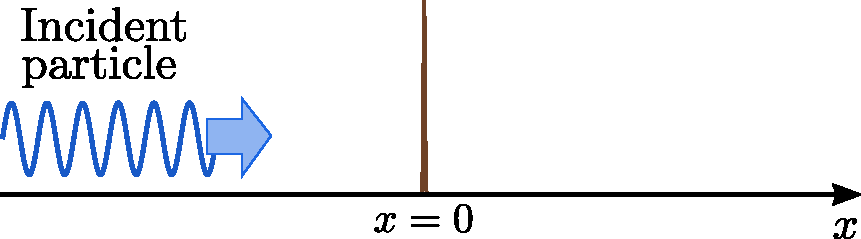
\includegraphics[width=0.45\textwidth]{scattering1d}
\end{figure}

If you are disturbed by the idea of a delta function potential, just
regard it as the limiting case of a family of increasingly tall and
narrow gaussian functions centered at $x=0$.  For non-singular
potentials, the validity of the Schr\"odinger wave equation relies on
$\psi(x)$ being continuous with well-defined first and second
derivatives.  In the delta function limit, however, these conditions
are relaxed: $\psi(x)$ remains continuous, but at $x=0$ its first
derivative becomes discontinuous.  To see this, integrate the
Schr\"odinger wave equation over an infinitesimal range around $x =
0$:
\begin{align}
  \begin{aligned}\lim_{\varepsilon\rightarrow 0^+} \int_{-\varepsilon}^{+\varepsilon} dx\; \left[-\frac{\hbar^2}{2m} \frac{d^2}{dx^2} + \frac{\hbar^2\gamma}{2m} \delta(x)\right] \psi(x) &= \lim_{\varepsilon\rightarrow 0^+} \int_{-\varepsilon}^{+\varepsilon} dx\; E \psi(x) \\ = \lim_{\varepsilon\rightarrow 0^+} \left\{-\frac{\hbar^2}{2m} \left[\frac{d\psi}{dx}\right]_{-\varepsilon}^{+\varepsilon} \right\} + \frac{\hbar^2\gamma}{2m} \psi(0) &= 0.
  \end{aligned}
\end{align}
Hence,
\begin{equation}
  \lim_{\varepsilon\rightarrow 0^+} \left\{\; \left.\frac{d\psi}{dx}\right|_{x = +\varepsilon} - \left.\frac{d\psi}{dx}\right|_{x = -\varepsilon}\; \right\} =  \gamma \,\psi(0).
  \label{delta_discontinuity}
\end{equation}

To proceed, consider a particle incident from the left, with energy
$E$.  This is described by an incident state proportional to a
momentum eigenstate $|k\rangle$, where $k = \sqrt{2mE/\hbar^2} > 0$.
We said ``proportional'', not ``equal'', for it is conventional to
adopt the normalization
\begin{equation}
  |\psi_i\rangle = \sqrt{2\pi}\Psi_i |k\rangle \;\;\; \Leftrightarrow\;\;\; \psi_i(x) = \langle x|\psi\rangle = \Psi_i \, e^{ik x},
\end{equation}
where the complex constant $\Psi_i$ is called the \textbf{incident
  amplitude}.  Plugging this back into the Schr\"odinger wave equation
yields
\begin{equation}
  \left[-\frac{\hbar^2}{2m} \frac{d^2}{dx^2} + \frac{\hbar^2\gamma}{2m}\delta(x)\right] \left(\Psi_i \, e^{ikx} + \psi_s(x) \right) = E \left(\Psi_i \, e^{ikx} + \psi_s(x) \right).
\end{equation}
Taking $E = \hbar^2k^2/2m$, and doing a bit of algebra, simplifies this to
\begin{equation}
  \left[ \frac{d^2}{dx^2} + k^2\right] \psi_s(x) =  \gamma \delta(x) \left(\Psi_i \, e^{ikx} + \psi_s(x) \right).
  \label{deltaschrod}
\end{equation}

We can construct the solution by separately considering the regions $x
< 0$ and $x > 0$.  Within each half-space, $\delta(x)$ vanishes so
Eq.~\eqref{deltaschrod} reduces to
\begin{equation}
  \left[\frac{d^2}{dx^2} + k^2\right] \psi_s(x) = 0.
\end{equation}
This called the \textbf{Helmholtz equation}.  It has a general
solution of the form
\begin{equation}
  \psi_s(x) = \Psi_i \left(f_1 \, e^{ik x} + f_2 \, e^{-ik x}\right),
\end{equation}
where $f_1$ and $f_2$ can take on different values in each region ($x
< 0$ or $x > 0$).

We want $\psi_s(x)$ to describe an \textbf{outgoing wave}, which means
it ought to be purely left-moving for $x < 0$, and purely right-moving
for $x > 0$.  Therefore, let $f_1 = 0$ for $x < 0$, and $f_2 = 0$ for
$x > 0$, so that
\begin{equation}
  \psi_s(x) = \Psi_i \times \begin{cases}f_- \,e^{-ikx}, & x < 0 \\ f_+ \,e^{ikx}, & x > 0.\end{cases}
\end{equation}
The complex numbers $f_-$ and $f_+$ are called \textbf{scattering
  amplitudes}.  They parameterize the magnitude and phase of the
scattered wavefunction moving outward from the scatterer.

Recall from the discussion at the beginning of this section that
$\psi(x)$ must be continuous everywhere, including at $x = 0$.  Since
$\psi_i(x)$ is continuous, $\psi_s(x)$ must be as well, so $f_- =
f_+$.  Moreover, we showed in Eq.~\eqref{delta_discontinuity} that the
first derivative of $\psi(x)$ is discontinuous at the scatterer.
Plugging \eqref{delta_discontinuity} into our expression for
$\psi(x)$, at $x = 0$, gives
\begin{equation}
  \Psi_i\big[ik(1+f_\pm) - ik(1-f_\pm)\big] =  \Psi(1+f_\pm) \gamma.
\end{equation}
Hence, we obtain
\begin{equation}
  f_+ = f_- = -\frac{\gamma}{\gamma - 2ik}.
\end{equation}

For now, let us focus on the magnitude of the scattering amplitude (in
the next chapter, we will see that the phase also contains useful
information).  The quantity $|f_\pm|^2$ describes the overall strength
of the scattering process:
\begin{equation}
  |f_\pm|^2 = \left[1 + \frac{8mE}{(\hbar\gamma)^2}\right]^{-1}.
\end{equation}
Its dependence on $E$ is plotted below:

\begin{figure}[h]
  \centering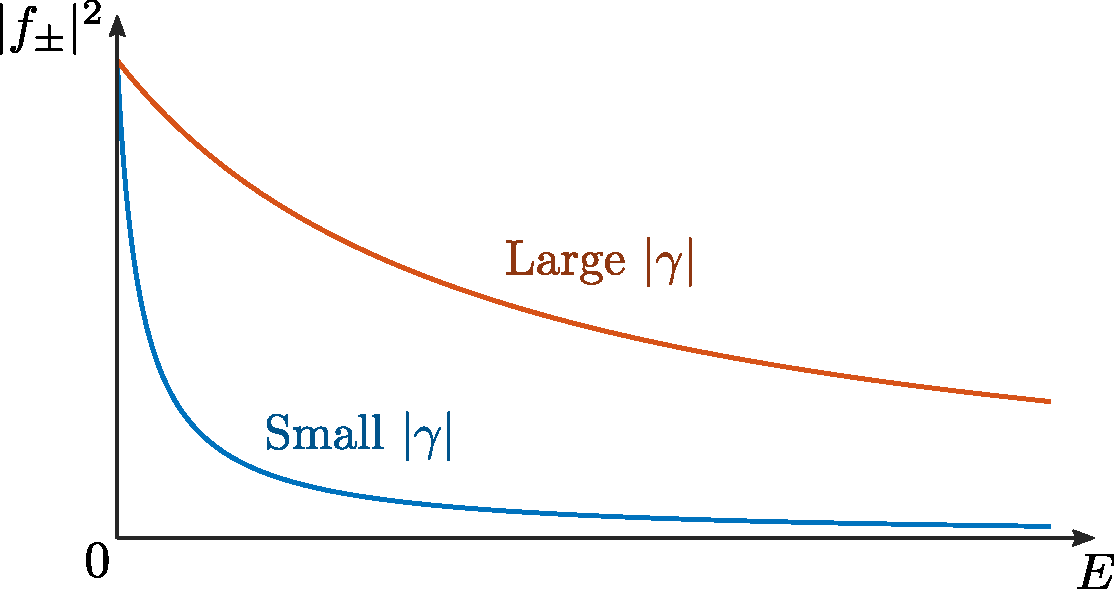
\includegraphics[width=0.55\textwidth]{scattering1df}
\end{figure}

\noindent
For fixed potential strength $\gamma$, we see that the scattering
strength decreases monotonically with $E$, meaning that higher-energy
particles are scattered less easily.  On the other hand, for fixed
$E$, the scattering strength increases with $|\gamma|$, with the limit
$|f|^2 \rightarrow 1$ as $|\gamma|\rightarrow \infty$.  Note also that
attractive potentials ($\gamma < 0$) and repulsive potentials ($\gamma
> 0$) are equally effective scatterers.

\section{Scattering in 2D and 3D}
\label{sec:2d3d_scattering}

We now consider scattering experiments in spatial dimension $d \ge 2$.
These have a new and important feature: for $d = 1$, the particle can
only scatter forward or backward, but for $d \ge 2$ it can be
scattered to the side.

Far from the scatterer, where $V(\mathbf{r})\rightarrow 0$, the
scattered wavefunction $\psi_s(\mathbf{r})$ satisfies
\begin{equation}
  -\frac{\hbar^2}{2m} \nabla^2 \psi_s(\mathbf{r}) = E \psi_s(\mathbf{r}),
\end{equation}
where $\nabla^2$ denotes the $d$-dimensional Laplacian.  Let $E =
\hbar^2 k^2 / 2m$, where $k \in \mathbf{R}^+$ is the wave-number in
free space.  Then the above equation can be written as
\begin{equation}
  \left[\nabla^2 + k^2\right] \psi_s(\mathbf{r}) = 0,
  \label{helmholtzeq}
\end{equation}
which is the \textbf{Helmholtz equation} in $d$-dimensional space.

We already know of one set of elementary solutions to
Eq.~\eqref{helmholtzeq}, the plane waves
\begin{equation*}
  \big\{\exp(i\mathbf{k}\cdot\mathbf{r}),\;\;\mathrm{where}\;\;
  |\mathbf{k}| = k \big\}.
\end{equation*}
However, we're looking for scattered wavefunctions that are outgoing
waves, and a plane wave can't be said to be ``outgoing''.  The
solution, as we shall see, is to construct solutions expressed in
curvilinear coordinates.

Take the 2D case first.  Skipping the mathematical details, one finds
that the general solution to Eq.~\eqref{helmholtzeq} in 2D can be
written, using polar coordinates $(r,\phi)$, as
\begin{equation}
  \psi(\mathbf{r})=\sum_{\pm}\sum_{m=-\infty}^\infty c_m^\pm\,\Psi_m^\pm(r,\phi), \;\;\;\mathrm{where}\;\;\,\Psi_m^\pm(r,\phi) = H_m^\pm(kr)\,e^{im\phi}.
\end{equation}
This is a superposition of circular waves $\Psi_m^\pm(r,\phi)$, with
coefficients $c_m^\pm \in \mathbb{C}$.  Each circular wave is a
solution to the 2D Helmholtz equation with angular momentum quantum
number $m \in \mathbb{Z}$.  Its $r$-dependence is given by $H_m^\pm$,
called a \textbf{Hankel function} of the ``first kind'' ($+$) or
``second kind'' ($-$).  Some Hankel functions of the first kind are
plotted below:

\begin{figure}[h!]
  \centering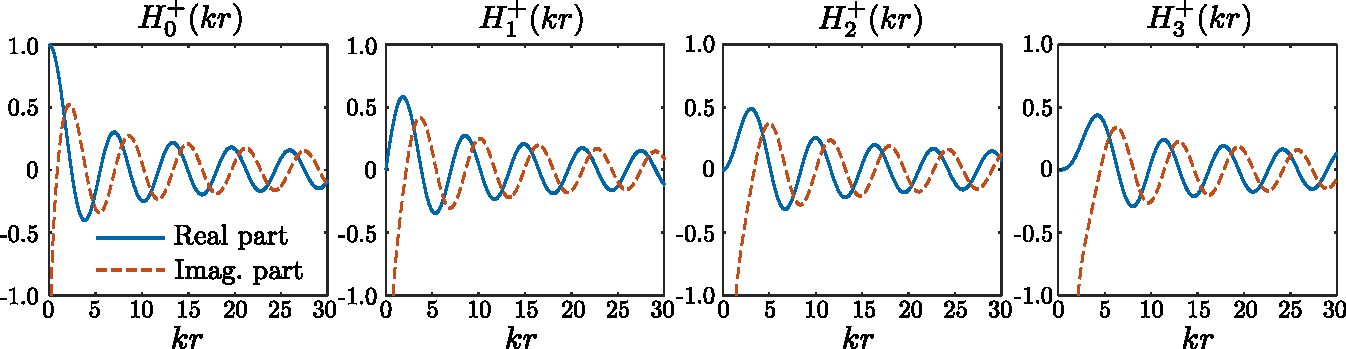
\includegraphics[width=0.95\textwidth]{besselh}
\end{figure}

The $H^-_m$ functions are the complex conjugates of $H^+_m$.  For
large values of the input,
\begin{equation}
  H_m^\pm(kr) \overset{r\rightarrow\infty}{\longrightarrow} \sqrt{\frac{2}{\pi kr}} \, \exp\left[\pm i\left(kr - \frac{(m+\frac{1}{2})\pi}{2}\right)\right] \;\sim\; r^{-1/2} e^{\pm ikr}.
\end{equation}
Therefore, the $\pm$ index specifies whether the circular wave is an
\textbf{outgoing wave} directed outward from the origin ($+$), or an
\textbf{incoming wave} directed toward the origin ($-$).

The 3D case is treated similarly.  We use spherical coordinates
$(r,\theta,\phi)$, and the solutions of the 3D Helmholtz equation are
superpositions of incoming and outgoing spherical waves:
\begin{equation}
  \psi(\mathbf{r})=\sum_{\pm}\sum_{\ell=0}^\infty\sum_{m=-\ell}^\ell c_{\ell m}^\pm \,\Psi_{\ell m}^\pm(r,\theta,\phi)\;\;\;\mathrm{where}\;\;\Psi_{\ell m}^\pm(r,\theta,\phi) = \,h_\ell^\pm(kr)\,Y_{\ell m}(\theta,\phi).
\end{equation}
The $c_{\ell m}^\pm$ factors are complex coefficients.  Each
$h_\ell^\pm$ is a \textbf{spherical Hankel function}, and each
$Y_{\ell m}$ is a \textbf{spherical harmonic}.  The $\ell$ and $m$
indices specify the angular momentum of the spherical wave.  For large
inputs, the spherical Hankel functions have the limiting form
\begin{equation}
  h_\ell^\pm(kr) \overset{r\rightarrow\infty}{\longrightarrow} \pm \frac{\exp\!\left[\pm i\!\left(kr-\frac{\ell\pi}{2}\right)\right]}{ikr}.
\end{equation}
Hence, the $\pm$ index specifies whether the spherical wave is
outgoing ($+$) or incoming ($-$).  More discussion about these
spherical waves can be found in Appendix A.

It is now clear what we need to do to get a scattered wavefunction
$\psi_s(\mathbf{r})$ that is outgoing at infinity.  We simply write it
as a superposition of only outgoing ($+$) waves:
\begin{equation}
  \psi_s(\mathbf{r}) = \begin{cases} \displaystyle\sum_{m} c_m^+\,H_m^+(kr)\,e^{im\phi}, &d=2\\ \displaystyle\sum_{\ell m} c_{\ell m}^+\,h_\ell^+(kr)\,Y_{\ell m}(\theta,\phi),&d=3.\end{cases}
\end{equation}
At large distances, the $r$-dependence reduces to
\begin{equation}
  \psi_s(\mathbf{r}) \; \overset{r\rightarrow\infty}{\sim} \; r^{\frac{1-d}{2}} \,\exp\left(ikr\right).
\end{equation}
For $d > 1$, the magnitude decreases with $r$, which is to be expected
since the outgoing wave spreads out over a wider area.  More
precisely, if we look at the probability current density
\begin{equation*}
  \mathbf{J} = (\hbar/m) \mathrm{Im}\left[\psi_s^*\nabla\psi_s\right],  
\end{equation*}
its $r$-component scales as
\begin{equation}
  \begin{aligned}J_r \; &\overset{r\rightarrow\infty}{\sim} \; \mathrm{Im}\left[r^{\frac{1-d}{2}} e^{-ikr} \frac{\partial}{\partial r}\left(r^{\frac{1-d}{2}} e^{ikr}\right)\right] \\ &\;\;=\;\;\;\mathrm{Im}\left[\frac{1-d}{2}\, r^{-d} + ik r^{1-d}\right]\\ &\;\;=\;\;\; k \,r^{1-d}.\end{aligned}
  \label{Jr}
\end{equation}
In $d$ dimensions, the area of a wave-front scales as $r^{d-1}$, so
the probability flux goes as $J_r \,r^{d-1} \sim k$, which is positive
and independent of $r$.  Hence, there is a constant probability flux
flowing outward from the origin.  Note that for $d=1$, Eq.~\eqref{Jr}
states that $J_r \sim r^0$, consistent with the results of the
previous section: in 1D, waves do not spread with distance since there
is no transverse dimension.

\section{The scattering amplitude and scattering cross section}
\label{sec:scattering_amplitude}

We can use the results of the previous section to express the outcomes
of a scattering experiment in a cleaner and more systematic way.
Consider an incident plane wave,
\begin{equation}
  \psi_i(\mathbf{r}) = \Psi_i \, e^{i\mathbf{k}_i\cdot\mathbf{r}},
\end{equation}
in $d$-dimensional space.  Here, $\Psi_i \in \mathbb{C}$ is the
\textbf{incident wave amplitude}, and $\mathbf{k}_i$ is the incident
momentum whose magnitude is $k = |\mathbf{k}_i|$, so that the particle
energy is $E = \hbar^2k^2/2m$.  We adopt coordinates $(r,\Omega)$,
where $r$ is the distance from the origin and $\Omega$ denotes the
other coordinates.  For 1D, $\Omega \in \pm$ specifies the choice of
``forward'' or ``backward'' scattering; for 2D polar coordinates,
$\Omega = \phi$; and for 3D spherical coordinates, $\Omega =
(\theta,\phi)$.

Far from the origin, the scattered wavefunction reduces to
\begin{equation}
  \psi_s(\mathbf{r})\;  \overset{r\rightarrow\infty}{\longrightarrow}\; \Psi_i \, r^{\frac{1-d}{2}} \, e^{ikr} \, f(\Omega).
\end{equation}
The complex function $f(\Omega)$, called the \textbf{scattering
  amplitude}, is the fundamental quantity of interest in scattering
experiments.  It describes how the particle is scattered in various
directions, depending on the inputs to the problem (i.e.,
$\mathbf{k}_i$ and the scattering potential).

Sometimes, we write the scattering amplitude using the alternative
notation
\begin{equation}
  f(\mathbf{k}_i \rightarrow \mathbf{k}_f), \;\;\;\mathrm{where}\;\; \mathbf{k}_f = k \hat{\mathbf{r}}.
\end{equation}
This emphasizes firstly that the incident wave-vector is
$\mathbf{k}_i$; and secondly that the particle is scattered in some
direction which can be specified by either the unit position vector
$\hat{\mathbf{r}}$, or equivalently by the momentum vector
$\mathbf{k}_f = k \hat{\mathbf{r}}$, or by the angular coordinates
$\Omega$.

From the scattering amplitude, we define two other important
quantities of interest:
\begin{framed}
  \begin{align}
    \frac{d\sigma}{d\Omega} &= \big|f(\Omega)\big|^2 \qquad\quad\quad \text{(the \textbf{differential scattering cross section})} \\ \sigma &= \int d\Omega\; \big|f(\Omega)\big|^2 \quad\; \text{(the \textbf{total scattering cross section}).} \label{sigma}
  \end{align}
\end{framed}
\vskip -0.05in
\noindent
In Eq.~\eqref{sigma}, $\int d\Omega$ denotes the integral(s) over all
the angle coordinates; for 1D, this is instead a discrete sum over the
two possible directions, forward and backward.

The term ``cross section'' comes from an analogy with the scattering
of classical particles.  Consider the probablity current density
associated with the scattered wavefunction:
\begin{equation}
  \mathbf{J}_s = \frac{\hbar}{m} \mathrm{Im}\big[\psi_s^*\nabla\psi_s\big].
\end{equation}
Let us focus only on the $r$-component of the current density, in the
$r\rightarrow\infty$ limit:
\begin{equation}
  \begin{aligned}J_{s,r}\; &\;\;=\;\;\;\, \frac{\hbar}{m}\, \mathrm{Im}\left[\psi_s^* \frac{\partial}{\partial r}\psi_s\right] \\ &\overset{r\rightarrow\infty}{\longrightarrow}\;\, \frac{\hbar}{m}\; |\Psi_i|^2 \; |f(\Omega)|^2 \mathrm{Im}\left[\left(r^{\frac{1-d}{2}} \, e^{ikr}\right)^* \frac{\partial}{\partial r} \left(r^{\frac{1-d}{2}} \, e^{ikr}\right)\right] \\ & \;\;=\;\;\;\, \frac{\hbar \,k}{m}\; |\Psi_i|^2 \; |f(\Omega)|^2 \,r^{1-d}.\end{aligned}
\end{equation}
The total flux of outgoing probability is obtained by integrating
$J_{s,r}$ over a constant-$r$ surface:
\begin{equation}
  I_s \;=\; \int d\Omega\; r^{d-1} \, J_{s,r} \;=\; \frac{\hbar k}{m} \;|\Psi_i|^2 \; \int d\Omega\; \big|f(\Omega)\big|^2.
  \label{scatterI}
\end{equation}
We can assign a physical interpretation to each term in this
result.  The first factor, $\hbar k/m$, is the
particle's speed (i.e., the group velocity of the de Broglie wave).
The second factor, $|\Psi_i|^2$, is the probability density of the incident
wave, which has units of $[x^{-d}]$ (i.e., inverse $d$-dimensional
``volume'').  The product of these two factors represents the
\textbf{incident flux},
\begin{equation}
  J_{i} = \frac{\hbar k}{m} \;|\Psi_i|^2.
\end{equation}
This has units of $[x^{1-d}t^{-1}]$ (i.e., rate per unit ``area'' in
$d$-dimensional space).

Let us re-imagine this incident flux $J_i$ as a stream of classical
particles, and the scatterer as a ``hard-body'' scatterer that only
interacts with those particles striking it directly:

\begin{figure}[h]
  \centering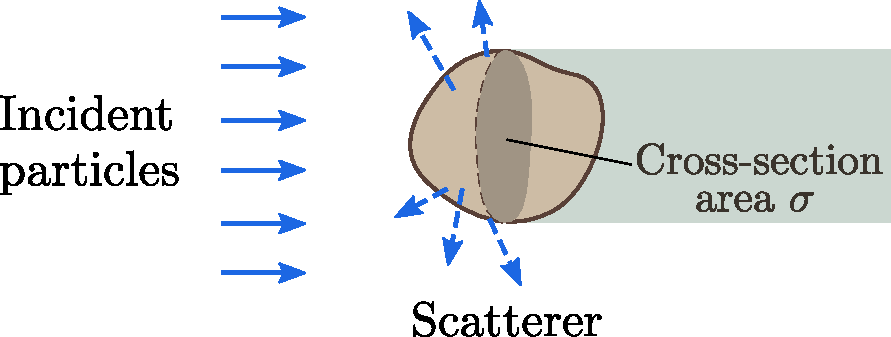
\includegraphics[width=0.44\textwidth]{crosssection}
\end{figure}

\noindent
In this classical picture, the rate at which the incident particles
strike the scatterer is
\begin{equation}
  I_s = J_i \, \sigma,
\end{equation}
where $\sigma$ is the exposed cross-sectional area of the scatterer.
Comparing this expression to Eq.~\eqref{scatterI}, we see that $\int
d\Omega\,|f|^2$ plays a role analogous to the classical hard-body
cross-sectional area.  We hence call
\begin{equation*}
  \sigma \equiv \int d\Omega\,|f|^2
\end{equation*}
the \textbf{total scattering cross section}.  Moreover, the integrand
$|f|^2$ is called the \textbf{differential scattering cross section},
for it represents the rate, per unit of solid angle, at which
particles are scattered in a given direction.  The total and
differential scattering cross sections are the principal observable
quantities that can be obtained from scattering experiments.

\section{The Green's function}
\label{sec:greensfun}

The scattering amplitude $f(\Omega)$ can be calculated using a variety
of analytical and numerical methods.  We will discuss one particularly
important approach, based on a quantum variant of the Green's function
technique for solving inhomogenous differential equations.

Let us return to the previously-discussed formulation of the
scattering problem:
\begin{align}
  \begin{aligned} \hat{H} &= \hat{H}_0+\hat{V} \\ \hat{H} |\psi\rangle &= E |\psi\rangle \\ |\psi\rangle &= |\psi_i\rangle \,+\, |\psi_s\rangle \\ \hat{H}_0 |\psi_i\rangle &= E |\psi_i\rangle.\end{aligned}
\end{align}
These equations can be combined as follows:
\begin{align}
  \begin{aligned} \left(\hat{H}_0 + \hat{V}\right) |\psi_i\rangle + \hat{H} |\psi_s\rangle &= E \left( |\psi_i\rangle + |\psi_s\rangle \right) \\ \Rightarrow \quad \hat{V} |\psi_i\rangle + \hat{H} |\psi_s\rangle &= E |\psi_s\rangle  \\ \Rightarrow \quad\; \left(E - \hat{H}\right) |\psi_s\rangle & = \hat{V} |\psi_i\rangle
  \end{aligned}
\end{align}
To proceed, we define the inverse of the operator on the left-hand
side:
\begin{equation}
  \hat{G} = \big(E-\hat{H}\big)^{-1}.
\end{equation}
This operator is called the \textbf{Green's function}.  Using it, we
get
\begin{equation}
  |\psi_s\rangle = \hat{G} \hat{V} |\psi_i\rangle.
  \label{scatterform}
\end{equation}

Note that $\hat{G}$ depends on both the energy $E$ and the scattering
potential.  To isolate the dependence on the scattering potential, let
us define the Green's function for a free particle,
\begin{equation}
  \hat{G}_0=\big(E-\hat{H}_0\big)^{-1}.
\end{equation}
This will be very useful for us, for $\hat{G}_0$ can be calculated
exactly, whereas $\hat{G}$ often has no analytic expression.  We can
relate $G$ and $G_0$ as follows:
\begin{align}
  \begin{aligned}
    \hat{G}(E-\hat{H}_0 - \hat{V})\;\; &= I \;\;\;\mathrm{and}\;\; (E-\hat{H}_0 - \hat{V})\hat{G} = I \\ \Rightarrow \;\;\; \hat{G} \hat{G}_0^{-1} - \hat{G}\hat{V} &= I \;\;\; \mathrm{and}\;\;\;\;\, \hat{G}_0^{-1} \hat{G} - \hat{V}\hat{G} \;\;\;= I.
  \end{aligned}
\end{align}
Upon respectively right-multiplying and left-multiplying these equations
by $\hat{G}_0$, we arrive at the following pair of equations, called
\textbf{Dyson's equations}:
\begin{framed}
  \begin{align}
    \hat{G} \;&= \; \hat{G}_0 + \hat{G}\hat{V}\hat{G}_0 \\
    \hat{G} \;&=\; \hat{G}_0 + \hat{G}_0\hat{V}\hat{G} \label{dyson2}
  \end{align}
\end{framed}
\noindent
These equations are ``implicit'', as the unknown $\hat{G}$ appears in
both the left and right sides.

Applying the second Dyson equation, Eq.~\eqref{dyson2}, to the
scattering problem \eqref{scatterform} gives
\begin{align}
  \begin{aligned}|\psi_s\rangle &= \left(\hat{G}_0 + \hat{G}_0\hat{V}\hat{G}\right) \hat{V} |\psi_i\rangle \\ &= \hat{G}_0 \hat{V} |\psi_i\rangle + \hat{G}_0\hat{V}\hat{G} \hat{V} |\psi_i\rangle \\ &= \hat{G}_0 \hat{V} |\psi_i\rangle + \hat{G}_0\hat{V} |\psi_s\rangle \\ &= \hat{G}_0\hat{V} |\psi\rangle.\end{aligned}
  \label{psis_implicity}
\end{align}
This is a useful simplification, since it involves $\hat{G}_0$ rather
than $\hat{G}$.  The downside is that the equation is still implicit:
the right-hand side involves the unknown total state $|\psi\rangle$,
rather than the known incident state $|\psi_i\rangle$.

We can try to solve the implicit equation by using
Eq.~\eqref{psis_implicity} to get an expression for $|\psi\rangle$,
then repeatedly plugging the result back into the right-hand side of
Eq.~\eqref{psis_implicity}:
\begin{align}
  \begin{aligned}|\psi_s\rangle &= \hat{G}_0 \hat{V} \left(|\psi_i\rangle + \hat{G}_0 \hat{V}|\psi\rangle\right) \\ &= \quad \vdots \\ &= \left[\hat{G}_0 \hat{V} + (\hat{G}_0 \hat{V})^2 + (\hat{G}_0 \hat{V})^3 + \cdots\right]|\psi_i\rangle.\end{aligned}
\end{align}
Or, equivalently,
\begin{equation}
  |\psi\rangle = \left[\hat{I} + \hat{G}_0 \hat{V} + (\hat{G}_0 \hat{V})^2 + (\hat{G}_0 \hat{V})^3 + \cdots\right]|\psi_i\rangle.
  \label{bornseries}
\end{equation}
This is called the \textbf{Born series}.

To interpret this result, let us go to the position basis:
\begin{align}
  \begin{aligned}\psi(\mathbf{r}) = \psi_i(\mathbf{r}) &+ \int d^dr' \langle \mathbf{r} | \hat{G}_0 |\mathbf{r}'\rangle\, V(\mathbf{r}') \psi_i(\mathbf{r}') \\ &+ \int d^dr' d^dr'' \langle \mathbf{r} | \hat{G}_0 |\mathbf{r}'\rangle\, V(\mathbf{r}') \, \langle \mathbf{r}' | \hat{G}_0 |\mathbf{r}''\rangle \, V(\mathbf{r}'') \psi_i(\mathbf{r}'') \\ &+ \;\;\cdots\end{aligned}
\end{align}
This formula can be regarded as a description of \textbf{multiple
  scattering}.  Due to the presence of the scatterer, the particle
wavefunction is a quantum superposition of terms describing zero, one,
two, or more scattering events, as illustrated below:

\begin{figure}[h!]
  \centering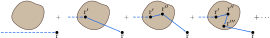
\includegraphics[width=0.98\textwidth]{bornseries}
\end{figure}

\noindent
Each successive term in the Born series involves more scattering
events, i.e., higher multiples of $\hat{V}$.  For example, the
second-order term is
\begin{equation*}
  \int d^dr' d^dr'' \langle \mathbf{r} | \hat{G}_0 |\mathbf{r}'\rangle\, V(\mathbf{r}') \, \langle \mathbf{r}' | \hat{G}_0 |\mathbf{r}''\rangle \, V(\mathbf{r}'') \psi_i(\mathbf{r}'').
\end{equation*}
This describes the particle undergoing (i) scattering of the incident
particle at point $\mathbf{r}''$, (ii) propagation from $\mathbf{r}''$
to $\mathbf{r}'$, (iii) scattering again at point $\mathbf{r}'$, and
(iv) propagation from $\mathbf{r}'$ to $\mathbf{r}$.  Note that
$\mathbf{r}'$ and $\mathbf{r}''$ are integrated over all possible
positions; since the integrals are weighted by $V$, the positions with
the strongest scattering potential contribute the most.

For a sufficiently weak scatterer, it is often a good approximation to
retain just the first few terms in the Born series.  However, the
question of what it means for $\hat{V}$ to be ``sufficiently
weak''---i.e., the exact requirements for the Born series to
converge---is a complex topic beyond the scope of our present
discussion.

\section{The Green's function for a free particle}
\label{sec:freegreen}

We have defined the free-particle Green's function as the operator
$\hat{G}_0=\big(E-\hat{H}_0\big)^{-1}$.  Its representation in the
position basis, $\langle\mathbf{r}|\hat{G}_0|\mathbf{r}'\rangle$, is
called the \textbf{propagator}.  As we have just seen, when the Born
series is written in the position basis, the propagator appears in the
integrand and describes how the particle ``propagates'' between
discrete scattering events.

The propagator is a solution to a partial differential equation:
\begin{align}
  \begin{aligned}\langle\mathbf{r} |\big(E-\hat{H}_0\big) \hat{G}_0 |\mathbf{r}'\rangle &= \langle\mathbf{r}|\hat{I}|\mathbf{r}'\rangle \\ = \left(E + \frac{\hbar^2}{2m}\nabla^2 \right) \langle\mathbf{r} |\hat{G}_0 |\mathbf{r}'\rangle &= \delta^d(\mathbf{r}-\mathbf{r}') \\ \Rightarrow \qquad\quad \left(\nabla^2 + k^2\right) \langle\mathbf{r} |\hat{G}_0 |\mathbf{r}'\rangle &= \frac{2m}{\hbar^2} \delta^d(\mathbf{r}-\mathbf{r}').\end{aligned}
\end{align}
As before, $k = \sqrt{2mE/\hbar^2}$ where $E$ is the energy of the
incident particle.  Therefore, up to a factor of $2m/\hbar^2$, the
propagator is the Green's function for the $d$-dimensional Helmholtz
equation (see Section~\ref{sec:2d3d_scattering}).  Note that the
$\nabla^2$ acts upon the $\mathbf{r}$ coordinates, not $\mathbf{r}'$.

To solve for $\langle\mathbf{r}|\hat{G}_0|\mathbf{r}'\rangle$, we can
use the momentum eigenstates:
\begin{align}
  \begin{aligned}\langle\mathbf{r}|\hat{G}_0|\mathbf{r}'\rangle &=
    \langle\mathbf{r}|\hat{G}_0 \Big(\int d^dk' |\mathbf{k}'\rangle\langle\mathbf{k}'| \Big) |\mathbf{r}'\rangle \\ &= \int d^dk' \; \langle\mathbf{r}|\mathbf{k}'\rangle \; \frac{1}{E-\frac{\hbar^2|\mathbf{k}'|^2}{2m}} \; \langle\mathbf{k}'|\mathbf{r}'\rangle \\ &= \frac{2m}{\hbar^2} \frac{1}{(2\pi)^d} \int d^dk' \; \frac{\exp\left[i\mathbf{k}' \cdot (\mathbf{r}-\mathbf{r}')\right]}{k^2-|\mathbf{k}'|^2}.\end{aligned}
  \label{rGr}
\end{align}
To proceed, we must specify the spatial dimension $d$.  Let us set $d
= 3$; the calculations for other $d$ are fairly similar.  To calculate
the integral over the 3D wave-vector space, we adopt spherical
coordinates $(k',\theta,\phi)$, with the coordinate axes aligned so
that $\mathbf{r}-\mathbf{r}'$ points along the $\theta=0$ direction.
We can now do the integral:
\begin{align*}
  \begin{aligned}\langle\mathbf{r}|\hat{G}_0|\mathbf{r}'\rangle &= \frac{2m}{\hbar^2} \frac{1}{(2\pi)^3} \int d^3k' \; \frac{\exp\left[i\mathbf{k}'\cdot (\mathbf{r}-\mathbf{r}')\right]}{k^2-|\mathbf{k}'|^2} \\ &= \frac{2m}{\hbar^2} \frac{1}{(2\pi)^3} \int_0^\infty dk' \int_0^\pi d\theta \int_{0}^{2\pi} d\phi \;{k'}^{2}\sin\theta\; \frac{\displaystyle \exp\left(ik'|\mathbf{r}-\mathbf{r}'|\cos\theta\right)}{k^2-{k'}^2} \\ &= \frac{2m}{\hbar^2} \frac{1}{(2\pi)^2} \int_0^\infty dk' \int_{-1}^1 d\mu \;{k'}^2\; \frac{\displaystyle \exp\left(ik'|\mathbf{r}-\mathbf{r}'|\mu\right)}{k^2-{k'}^2} \qquad(\text{letting}\;\mu = \cos\theta) \\ &= \frac{2m}{\hbar^2} \frac{1}{(2\pi)^2} \int_0^\infty dk' \; \frac{ {k'}^2}{k^2-{k'}^2}\, \frac{\displaystyle \exp\left(ik'|\mathbf{r}-\mathbf{r}'|\right) - \exp\left(-ik'|\mathbf{r}-\mathbf{r}'|\right)}{ik'|\mathbf{r}-\mathbf{r}'|} \\ &= \frac{2m}{\hbar^2} \frac{1}{(2\pi)^2} \frac{i}{|\mathbf{r}-\mathbf{r}'|} \int_{-\infty}^\infty dk' \; \frac{\displaystyle k'\, \exp\left(ik'|\mathbf{r}-\mathbf{r}'|\right)}{(k' - k)(k'+k)}\end{aligned}
\end{align*}
This looks like something we can handle with contour integration
techniques.  But there's a snag: the integration contour runs over the
real-$k'$ line, and since $k \in \mathbb{R}^+$, there are two poles
on the contour (at $\pm k$).  Hence, the value of the integral, as
written, is singular.

To make the integral non-singular, we must ``regularize'' it by
tweaking its definition.  One way is to displace the poles
infinitesimally in the complex $k'$ plane, shifting them off the
contour.  We have a choice of whether to move each pole upwards or
downwards; this choice turns out to be linked to whether the waves
described by $\hat{G}_0$ are incoming, outgoing, or behave some other
way at infinity.  It turns out that the right choice for us is to move
the pole at $-k$ infinitesimally downwards, and the pole at $+k$
infinitesimally upwards:

\begin{figure}[h!]
  \centering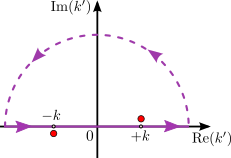
\includegraphics[width=0.37\textwidth]{greencontour}
\end{figure}

\noindent
This means replacing the denominator of the integrand as
follows:
\begin{equation}
  (k' - k)(k'+k) \;\rightarrow\; (k' - k - i\varepsilon)(k'+k+i\varepsilon) = {k'}^2 - (k+i\varepsilon)^2,
\end{equation}
where $\varepsilon$ is a positive infinitesimal.  This is equivalent
to replacing $E \rightarrow E + i\varepsilon$ in the definition of the
Green's function.  The integral can now be computed as
follows:
\begin{align*}
  \begin{aligned}\int_{-\infty}^\infty dk' \; \frac{\displaystyle k' \exp\left(ik'|\mathbf{r}-\mathbf{r}'|\right)}{(k' - k)(k'+k)} &\rightarrow \lim_{\varepsilon \rightarrow 0^+} \int_{-\infty}^\infty dk' \; \frac{\displaystyle k' \exp\left(ik'|\mathbf{r}-\mathbf{r}'|\right)}{(k' - k - i\varepsilon)(k'+k+i\varepsilon)}\;\;\; (\text{regularize}) \\ &= \lim_{\varepsilon \rightarrow 0^+} \int_C dk' \; \frac{\displaystyle k' \exp\left(ik'|\mathbf{r}-\mathbf{r}'|\right)}{(k' - k - i\varepsilon)(k'+k+i\varepsilon)} \quad\;\;\; (\text{close contour above}) \\ &= 2\pi i \lim_{\varepsilon \rightarrow 0^+} \mathrm{Res}\left[\frac{\displaystyle k' \exp\left(ik'|\mathbf{r}-\mathbf{r}'|\right)}{(k' - k - i\varepsilon)(k'+k+i\varepsilon)}\right]_{k'=k+i\varepsilon^+} \\ &= \pi i \exp\left(ik|\mathbf{r}-\mathbf{r}'|\right).\end{aligned}
\end{align*}
Plugging this into Eq.~\eqref{rGr} yields the propagator
$\langle\mathbf{r}|\hat{G}_0|\mathbf{r}'\rangle$.  The final result is
given below, along with the results for $d=1$ and $d=2$ (which are
obtained in a similar fashion):
\begin{framed}
  \begin{equation}
    \langle\mathbf{r}|\hat{G}_0|\mathbf{r}'\rangle = \frac{2m}{\hbar^2} \times \begin{cases} \Bigg.\displaystyle\frac{1}{2ik} \exp\left(ik|x-x'|\right),& d=1\\ \Bigg. \displaystyle\frac{1}{4i} H^+_0(k|\mathbf{r}-\mathbf{r'}|), & d=2 \\ \displaystyle \Bigg. - \frac{\exp\left(ik|\mathbf{r}-\mathbf{r}'|\right)}{4\pi|\mathbf{r}-\mathbf{r}'|}, & d = 3.  \end{cases}
  \end{equation}
\end{framed}

\vskip -0.15in
The propagator can be regarded as a function of the position
$\mathbf{r}$, describing a wave propagating outwards from a source
point $\mathbf{r}'$.  This outgoing behavior comes from our above
choice of regularization, which tweaked the definition of the Green's
function to be
\begin{framed}
  \begin{equation}
    \hat{G_0} = \lim_{\varepsilon\rightarrow 0^+} \big(E - \hat{H}_0 + i \varepsilon\big)^{-1}.
  \end{equation}
\end{framed}
\vskip -0.15in
\noindent
This is called an \textbf{outgoing} or \textbf{causal Green's
  function}.  The word ``causal'' refers to the concept of
``cause-and-effect'': i.e., a source at one point of space (the
``cause'') leads to the emission of waves that move outwards (the
``effect'').

Different regularizations produce Green's functions with alternative
features.  For instance, we could flip the sign of $i\varepsilon$ in
the Green's function redefinition, which displaces the $k$-space poles
in the opposite direction.  The resulting propagator
$\langle\mathbf{r}|\hat{G}_0|\mathbf{r}'\rangle$ is
complex-conjugated, and describes a wave moving inwards from infinity,
``sinking'' into the point $\mathbf{r}'$.  Such a choice of
regularization thus corresponds to an \textbf{incoming Green's
  function}.  In the scattering problem, we will always deal with the
outgoing/causal Green's function.

\section{Scattering amplitudes in 3D}
\label{sec:3damp}

The propagator can now be plugged into the scattering problem
posed in Sections~\ref{sec:scattering_amplitude}--\ref{sec:greensfun}:
\begin{align}
  \begin{aligned} \psi_i(\mathbf{r}) &= \Psi_i \, e^{i\mathbf{k}\cdot\mathbf{r}}, \\ \psi_s(\mathbf{r}) &= \langle\mathbf{r}| \hat{G}_0 \hat{V} |\psi\rangle \;\; \overset{r\rightarrow\infty}{\longrightarrow}\;\; \Psi_i \, r^{\frac{1-d}{2}} \, e^{ikr} \, f(\mathbf{k}_i\rightarrow k\hat{\mathbf{r}}).
  \end{aligned}
\end{align}
Our goal is to determine the scattering amplitude $f$.  We will focus
on the 3D case; the 1D and 2D cases are handled in a similar way.

In the $r\rightarrow\infty$ limit, the propagator can be simplified
using the Taylor expansion
\begin{equation}
  |\mathbf{r} - \mathbf{r}'| = r - \hat{\mathbf{r}} \cdot \mathbf{r}' + \cdots,
\end{equation}
where $\hat{\mathbf{r}}$ denotes the unit vector pointing parallel to
$\mathbf{r}$.  (This is the same ``large-$r$'' expansion used in
deriving the electric dipole moment in classical electromagnetism.)
Applying this to the 3D outgoing propagator gives, to lowest order,
\begin{equation}
  \langle\mathbf{r}|\hat{G}_0|\mathbf{r}'\rangle \overset{r\rightarrow\infty}{\approx} - \frac{2m}{\hbar^2}\, \frac{e^{ikr}}{4\pi r}\; \exp\left(-ik \, \hat{\mathbf{r}} \cdot \mathbf{r}'\right)
\end{equation}
Hence, the scattered wavefunction is
\begin{align}
  \begin{aligned}\psi_s(\mathbf{r}) &\;\;= \;\; \int d^3r'\; \langle\mathbf{r}|\hat{G}_0|\mathbf{r}'\rangle\, V(\mathbf{r}')\, \psi(\mathbf{r}') \\ &\overset{r\rightarrow\infty}{\approx} \, - \frac{2m}{\hbar^2} \, \frac{e^{ikr}}{4\pi r}\; \int d^3r' \exp\left(-ik \, \hat{\mathbf{r}} \cdot \mathbf{r}'\right)\, V(\mathbf{r}')\, \psi(\mathbf{r}') \\ &\;\;=\;\; - \frac{2m}{\hbar^2} \, \frac{e^{ikr}}{4\pi r} \; (2\pi)^{3/2} \; \big\langle \mathbf{k}_f \big|\hat{V}\big|\psi\big\rangle, \;\;\;\mathrm{where}\;\; \mathbf{k}_f \equiv k \hat{\mathbf{r}}. \end{aligned}
\end{align}
We can combine this with the Green's function relation from
Section~\ref{sec:greensfun},
\begin{equation}
  |\psi\rangle = \left(\hat{I} + \hat{G}\hat{V}\right)|\psi_i\rangle.
\end{equation}
This yields
\begin{align}
  \begin{aligned}\psi_s(\mathbf{r}) \; &\overset{r\rightarrow\infty}{\longrightarrow} \; - \frac{2m}{\hbar^2} \, \frac{e^{ikr}}{r} \; \sqrt{\frac{\pi}{2}} \; \big\langle \mathbf{k}_f \big|\hat{V} + \hat{V}\hat{G}\hat{V}\big|\psi_i\big\rangle \\ &= - \frac{2m}{\hbar^2} \, \Psi_i\, \frac{e^{ikr}}{r} \; 2\pi^2 \; \big\langle \mathbf{k}_f \big|\hat{V} + \hat{V}\hat{G}\hat{V}\big|\mathbf{k}_i\big\rangle.\end{aligned}
\end{align}
This can be compared to the earlier definition of the scattering amplitude,
\begin{equation}
  \psi_s(\mathbf{r}) \; \overset{r\rightarrow\infty}{\longrightarrow} \; \Psi_i \frac{e^{ikr}}{r} f(\mathbf{k}_i\rightarrow \mathbf{k}_f ).
\end{equation}
Hence,
\begin{framed}
  \begin{align}
    \begin{aligned}
      f(\mathbf{k}_i \rightarrow \mathbf{k}_f) &= - \frac{2m}{\hbar^2} \,\cdot \, 2\pi^2 \; \big\langle \mathbf{k}_f\big| \hat{V} + \hat{V}\hat{G} \hat{V} \big|\mathbf{k}_i\big\rangle \\
      &= - \frac{2m}{\hbar^2} \,\cdot \, 2\pi^2 \; \big\langle \mathbf{k}_f\big| \hat{V} + \hat{V}\hat{G}_0 \hat{V} + \hat{V} \hat{G}_0 \hat{V} \hat{G}_0\hat{V} + \cdots \big|\mathbf{k}_i\big\rangle,  \end{aligned}
  \end{align}
\end{framed}
\vskip -0.15in
\noindent
subject to the elasticity constraint $|\mathbf{k}_i| =
|\mathbf{k}_f|$.  In deriving the last line, we used the Born series
formula \eqref{bornseries}.

This result is the culmination of the numerous definitions and
derivations from the preceding sections.  On the left side is the
scattering amplitude, the fundamental quantity of interest in
scattering experiments.  The right side contains quantities that are
known to us, or that can be calculated: the initial and final momenta,
the scattering potential, and the Green's function.  Although this
result was derived for the 3D case, very similar formulas hold for
other dimensions, but with the $2\pi^2$ factor replaced with other
numerical factors.

\section{Example: uniform spherical well in 3D}

Let us test the Born series against a simple example, consisting of
the scattering potential
\begin{equation}
  V(\mathbf{r}) = \begin{cases}-U, & |\mathbf{r}| \le R \\ \;\;\;\,0,
    & |\mathbf{r}| > 0. \end{cases}
\end{equation}
We will assume that $U > 0$, so that the potential is attactive and
describes a uniform spherically symmetric well of depth $U$ and radius
$R$, surrounded by empty space.  For this potential, the scattering
problem can be solved exactly, using the method of \textbf{partial
  wave analysis} described in Appendix A.  The resulting scattering
amplitudes are
\begin{equation}
  \begin{aligned}f(\mathbf{k}_i \rightarrow \mathbf{k}_f) &= \frac{1}{2ik}\, \sum_{\ell =0}^\infty \big(e^{2i\delta_\ell} - 1\big) \big(2\ell+1\big)\, P_{\ell}(\hat{\mathbf{k}}_i\cdot \hat{\mathbf{k}}_f), \\ \mathrm{where}\;\; \delta_\ell &= \frac{\pi}{2} + \mathrm{arg}\!\left[k {h_\ell^+}'(kR) \, j_\ell(qR) - qh_\ell^+(kR)\, j_\ell'(qR)\right], \\ q &= \sqrt{2m(E+U)/\hbar^2} \\ k &\equiv |\mathbf{k}_i| = |\mathbf{k}_f|.\end{aligned}
\end{equation}
This solution is expressed in terms of various special functions;
$j_\ell$ and $h_\ell$ are the spherical Bessel function of the first
kind and spherical Hankel function, while $P_\ell$ is the
\href{https://en.wikipedia.org/wiki/Legendre_polynomials}{\textbf{Legendre
    polynomial}} (which appears in the definition of the spherical
harmonic functions).

We will pit this exact solution against the results from the Born
series:
\begin{equation}
  f(\mathbf{k}_i\rightarrow \mathbf{k}_f) \approx - \frac{2m}{\hbar^2} \,\cdot \, 2\pi^2 \, \Bigg[\big\langle \mathbf{k}_f\big| \hat{V}|\mathbf{k}_i\big\rangle + \big\langle \mathbf{k}_f \big| \hat{V}\hat{G}_0 \hat{V} \big|\mathbf{k}_i\big\rangle + \cdots \Bigg].
\end{equation}
The bra-kets can be evaluated in the position representation.  Let us
do this for just the first two terms in the series:
\begin{align*}
  \begin{aligned}f(\mathbf{k}_i\rightarrow \mathbf{k}_f) &\approx - \frac{2m}{\hbar^2} \; 2\pi^2 \Bigg[\int d^3r_1\; \frac{\exp(-i\mathbf{k}_f \cdot \mathbf{r}_1)}{(2\pi)^{3/2}} \, V(\mathbf{r}_1) \, \frac{\exp(i\mathbf{k}_i \cdot \mathbf{r}_1)}{(2\pi)^{3/2}} \\&\qquad\qquad\quad + \int d^3r_1 \!\! \int d^3r_2 \; \frac{\exp(-i\mathbf{k}_f \cdot \mathbf{r}_2)}{(2\pi)^{3/2}} \, V(\mathbf{r}_2) \, \langle\mathbf{r}_2|\hat{G}_0|\mathbf{r}_1 \rangle \, V(\mathbf{r}_1)\, \frac{\exp(i\mathbf{k}_i \cdot \mathbf{r}_1)}{(2\pi)^{3/2}}\Bigg] \\ &= \frac{1}{4\pi} \Bigg[\frac{2mU}{\hbar^2} \int_{|\mathbf{r}_1| \le R} d^3r_1 \; \exp\left[i(\mathbf{k}_i-\mathbf{k}_f)\, \cdot\, \mathbf{r}_1\right] \\ &\qquad + \left(\frac{2mU}{\hbar^2}\right)^2\, \int_{|\mathbf{r}_1|<R} d^3 r_1 \int_{|\mathbf{r}_2|<R} d^3 r_2 \; \frac{\exp\left[i(k|\mathbf{r}_1-\mathbf{r}_2| - \mathbf{k}_f \cdot \mathbf{r}_2 +\mathbf{k}_i \cdot \mathbf{r}_1)\right]}{4\pi|\mathbf{r}_1-\mathbf{r}_2|} \Bigg]. \end{aligned}
\end{align*}
If we use only the first term in the Born series, the result is
called the ``first Born approximation''; if we use two terms, the
result is called the ``second Born approximation''.  Higher-order Born
approximations can be derived in a similar fashion.

The most expedient way to calculate these integrals is to use
\href{https://en.wikipedia.org/wiki/Monte_Carlo_integration}{Monte
  Carlo integration}.  To find an integral of the form
\begin{equation}
  I = \int_{|\mathrm{r}|<R} d^3r \, F(\mathbf{r}),
\end{equation}
we randomly sample $N$ points within a cube of volume $(2R)^3$
centered around the origin, enclosing the desired sphere of radius
$R$.  For the $n$-th sampled point, $\mathbf{r}_n$, we compute
\begin{equation}
  F_n = \begin{cases}F(\mathbf{r}_n), & |\mathbf{r}| < R \\ 0, &\mathrm{otherwise}.\end{cases}
\end{equation}
The $F_n$'s give the values of the integrand at the sampling points,
omitting the contribution from points outside the sphere.  Then we
estimate the integral as
\begin{equation}
  I \,\approx\, (2R)^3 \, \langle F_n\rangle \,=\, \frac{(2R)^3}{N} \sum_{n=1}^N F_n.
\end{equation}
The estimate converges to the true value as $N\rightarrow\infty$; in
practice, $N \sim 10^4$ yields a good result for typical 3D integrals,
and can be computed in around a second on a modern computer.
Similarly, to calculate the double integral appearing in the second
term of the Born series, we sample \textit{pairs} of points; the
volume factor $(2R)^3$ is then replaced by $(2R)^6$.

This method for calculating the Born series can be readily generalized
to more complicated scattering potentials, including potentials for
which there is no exact solution.

The figure below shows the results of the Born approximation for the
uniform potential well, compared to the ``exact'' solution computed
from partial wave analysis.  It plots $|f|^2$ versus the scattering
energy $E$, for the case of $90^\circ$ scattering (i.e.,
$\mathbf{k}_f$ perpendicular to $\mathbf{k}_i$), with wells of
different depth $U$ and the same radius $R = 1$.  We adopt
computational units $\hbar = m = 1$, and each Monte Carlo integral is
computed using $3\times10^4$ samples.

\begin{figure}[h]
  \centering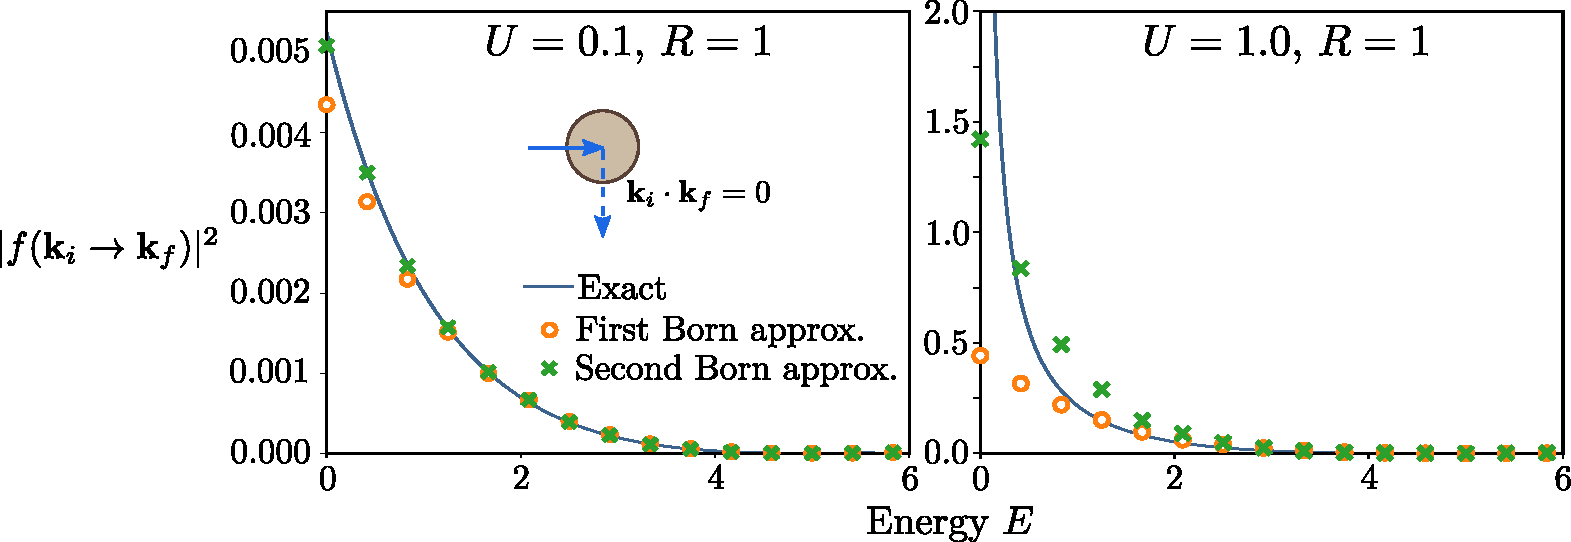
\includegraphics[width=0.97\textwidth]{spherical_well_scattering}
\end{figure}

The first thing to notice in these results in that $|f|^2$ diminishes
to zero for large $E$.  This makes sense, since the scattering
potential has some energy scale ($U$), so a incident particle that is
too energetic ($E \gg U$) will just zoom through, with little chance
of being deflected.

Looking more closely at the plots, we see that for the shallower well
($U = 0.1$), the first Born approximation agrees well with the exact
results, and the second Born approximation is even better,
particularly for small $E$.  For the deeper well ($U = 1$), the Born
approximations do not match the exact results.  Roughly speaking, for
the stronger scattering potential, an incident particle has a higher
chance to undergo multiple-scattering (i.e., bouncing around the
potential multiple times before escaping), which means that higher
terms in the Born series become more important.  In fact, if the
potential is too strong, taking the Born approximation to higher
orders might not even work, as the Born series itself can become
non-convergent.  In those cases, different methods must be brought to
bear.  We will see an example in the next chapter, in the form of
phenomena known as ``scattering resonances''.

\section*{Exercises}

\begin{enumerate}
\item In Sec.~\ref{sec:waves}, we derived the eigenstates of a
  particle in an empty infinite space by considering a box of length
  $L$ on each side, applying periodic boundary conditions, and taking
  $L \rightarrow \infty$.  Suppose we instead use Dirichlet boundary
  conditions (i.e., the wavefunction vanishes on the walls of the
  box).  Show that this gives rise to the same set of momentum
  eigenstates in the $L \rightarrow \infty$ limit.

\item Using the results for the 1D delta-function scattering problem
  described in Section~\ref{sec:1dscatter}, calculate the probability
  current
  \begin{equation}
    J(x) = \frac{\hbar}{2mi}\left(\psi^*\frac{d\psi}{dx} - \psi\frac{d\psi^*}{dx}\right),
  \end{equation}
  where $\psi(x)$ is the \textit{total} (incident + scattered)
  wavefunction.  Explain the relationship between the values of $J$ on
  the left and right side of the scatterer.

\item Derive the Green's function for a free particle in 1D space:
  \begin{equation}
    \langle x|\hat{G}_0|x'\rangle = \frac{2m}{\hbar^2} \cdot \frac{1}{2ik_i} \exp\left(ik_i|x-x'|\right).
  \end{equation}

\item In Section~\ref{sec:3damp}, the scattering amplitude
  $f(\mathrm{k}\rightarrow\mathrm{k}')$ for the 3D scattering problem
  was derived using the Born series.  Derive the corresponding
  expressions for 1D and 2D.
\end{enumerate}

\section*{Further Reading}

\begin{enumerate}[[1{]}]
\item Bransden \& Joachain, \S13.1---13.3 and \S13.5---13.6.
\item Sakurai, \S7.1--7.3, 7.5--7.6
\end{enumerate}

\end{document}


%% For decades after the discovery of quantum mechanics, the quantum
%% double-slit experiment was just a ``thought experiment'', meant to
%% illustrate the features of quantum mechanics that had been uncovered
%% by other, more complicated experiments.  Nowadays, the most convenient
%% way to do the experiment is with light, using single-photon sources
%% and single-photon detectors.  Quantum interference has also been
%% demonstrated experimentally using electrons, neutrons, and even
%% large-scale particles such as buckyballs.
